\yesmargins
\chapter{Unified Modeling Language (UML) Class and Sequence Diagrams}
\chaptermark{UML Diagrams}

\begin{tikzpicture}[overlay,remember picture] 
\node[anchor=south] at ([yshift=5in,xshift=0.8in]current page text area.south){\includegraphics[width=9in]{uml}}; 
\end{tikzpicture} 

\marginpar{
``Nobody, not even the creators of the UML, understand or use all of it.''
\begin{flushright}
\textit{Martin Fowler\\UML Distilled (3rd Ed.)}
\end{flushright}
}

After a discussion of diagrams in general, this chapter covers two common diagram types: UML class and sequence diagrams.

\section{How Diagrams Help}

Diagrams can help in at least two major ways:

\begin{enumerate}
\item {
They can \textbf{help you plan software} you will create.

Once you've created diagrams for planning your software, you can use them to communicate to the development team what will/should be implemented and decide (evaluate) whether your plans are any good (e.g., are clear, are logical, reflect your project's desired quality attributes, etc.).
}
\item {
They can \textbf{help you describe software} you've already created.

\marginpar{\classDiagramDef\margindivider}\marginpar{\sequenceDiagramDef\margindivider}If your software is already created, diagrams are good for documentation and, as mentioned above, for evaluating how satisfactory your software is.  The purpose of including diagrams in documentation is to communicate something about your software to somebody. There are many different audiences you could be trying to communicate with.
}
\end{enumerate}

\marginpar{Audiences often have short attention spans.\margindivider}Example audiences for your diagrams: Other developers on the project, your supervisor or manager, developers who might be interested in joining the team, developers who want to integrate with your system, curious end users, and students of software engineering.

Depending on the \textbf{IDE}\marginpar{\ideDef}/tools you're using, diagrams can be automatically generated from your code, which helps make documentation maintenance easier and  more likely to happen.

\section{What Diagrams Must Do Well}
To be helpful, diagrams must communicate \textbf{clearly} and at an \textbf{appropriate level of detail} for your intended audience. If your intended audience does not understand your diagram---or misunderstands it---your diagram has failed.

\section{What is UML?}

\textbf{UML (Unified Modeling Language)}\marginpar{\umlDef}\index{UML} is a family of graphical notations for describing and designing software through diagrams. It is especially applicable to object-oriented software, but some parts of UML are applicable to many types of software. Different UML notations are used for different types of UML diagrams, each of which have a specific purpose. UML was first published in 1994, became a standard of the Object Management Group (OMG) in 1997, and became an ISO standard in 2005. UML is currently on version 2.

\section{Why use UML?}

There are multiple \textbf{benefits} of creating diagrams using UML:\\

\begin{itemize}
\item UML gives you (1) \textbf{notation for designing} software so that your implementation will be structured and (2) \textbf{notation for describing} the existing design of software so that you can evaluate whether the design is any good.\\
\item UML diagramming \textbf{forces you to think} about software design in a structured way. When people try to design software in their minds, they can be sloppy about it---thinking about the aspects of the design they want to think about. UML can encourage you to face the more tricky parts of software design.\\
\item UML diagramming gives you a view of the software at \textbf{different levels of design} (e.g., class-level, component-level, package-level).\marginpar{Some IDEs will automatically generate some types of UML diagrams from your code. This is nice because it's easy to re-generate your diagram when your code changes. However, the generated diagrams can sometimes have more detail than you want, making them less good for communicating.}\\
\item UML provides a \textbf{common language} between software professionals. Because UML is well-known, it gives developers and managers a common vocabulary for communicating about software. That being said, expect to encounter some variation in how UML notation is used---it can be difficult to remember all the details of UML notations; many developers will make mistakes or adapt the notation to their own way of thinking. That is ok to do so long as you provide a legend or explanation of what your notation means.\\
\item UML diagrams give you a way to tell people about your software's structure \textbf{without asking them to look through code}. This is nice, for example, when onboarding new developers or communicating with managers.
\end{itemize}
\nomargins
\section{Why NOT use UML?}

There are also \textbf{drawbacks} to UML diagramming:\\

\begin{itemize}
\item People tend to \textbf{vary their UML notation}, which can cause \textbf{confusion}. Tips for avoiding that problem: (1) Keep your notation basic and (2) explain more complex notation usage to the people you're trying to communicate with.\\
\item Trying to get the UML notation details right \textbf{can take a lot of time}. Remember that diagrams are for communicating; If creating the diagram takes longer than explaining the code a different way, the diagram isn't helping.\\
\item UML diagrams \textbf{can require a lot of maintenance}. If your software design changes frequently, so must your UML diagrams if you want them to be accurate. Fortunately, some IDEs can generate some UML diagrams from your code.
\end{itemize}

\section{Class Diagrams}

A \textbf{class diagram}\index{class diagram} describes types of objects in a system and the static relationships that exist among them. Class diagrams also show properties and operations of a class and constraints on how objects are connected. UML uses the term ``feature'' as a general term that covers properties and operations of a class.\\

\noindent\textbf{Example class diagram:}
\begin{center}
\includegraphics[width=0.6\textwidth]{uml-classdiagram}
\end{center}

This class diagram shows the relationships between three classes: Customer, Order, and SharedOrder. An Order has one Customer---but the same Customer can be on multiple Orders. A SharedOrder is a type of Order that can have multiple Customers. The classes have ``attributes'' (e.g., id) and ``operations'' (e.g., getId()).

The next page explains each of the notational elements shown in the example. Class diagram notations gets more complicated than is described here; see publications in Additional Resources.

\subsection{UML Class Diagram Notation}
Below is a subset of UML class diagram notation. Some of the other notation tends to be confusing and so more people get it wrong (leading to miscommunication). However, if you'd like to learn about it anyway, see the references section at the end of this chapter.

\rowcolors{2}{gray!25}{white}
\noindent\begin{tabular}{p{2.5in} p{1in} p{2.5in}}
\rowcolor{gray!50}
Graphical Representation & Name & Description\\
\raisebox{-\totalheight}{\includegraphics[width=1in]{uml-note}} & note & A note. Notes are for putting comments on diagrams.\\
\raisebox{-\totalheight}{\includegraphics[width=2in]{uml-class2}} & class &  A class, potentially with attributes and operations (methods). The + indicates a public method, - is private, and \# is protected. The notation includes attribute types (e.g., int, Token, etc.), method parameters and return types, and default values for attributes.\\
\raisebox{-\totalheight}{\includegraphics[width=2.5in]{uml-association2}} & association & Association means that a class contains a reference to an object(s) of the other class in the form of an attribute. If Class1 points to Class2, Class1 \textit{has a} Class2.\\
\raisebox{-\totalheight}{\includegraphics[width=1in]{uml-generalization}} & inheritance & Inheritance means that one class is a subclass of another. If Class2 points to Class1, Class2 \textit{is a} Class1.\\
\raisebox{-\totalheight}{\includegraphics[width=2.5in]{uml-multiplicity}} & multiplicity & Multiplicity constrains the number of objects. If, for example, Class1 has three objects of type Class2, that's indicated with a 3 near the arrow pointing to Class2. 0..* (or just *) means zero or more. An integer N (e.g., 1) means exactly N. N..M means N to M (inclusive).\\
\end{tabular}

\yesmargins
\section{Sequence Diagrams}

A \textbf{sequence diagram}\marginpar{\sequenceDiagramDef\margindivider}\index{sequence diagram} describes interactions between objects. Usually, the diagram is showing a single use case or scenario. Sequence diagrams are a type of \textbf{interaction diagram}\marginpar{\interactionDiagramDef}\index{interaction diagram} and are not as good for showing object implementation details.

This section shows an example of a sequence diagram and commonly-used sequence diagram notation. To see more obscure notation, check the publications in the Additional Resources section.

\spacer
\noindent\textbf{Example sequence diagram:}

\begin{centering}
\includegraphics[width=\textwidth]{uml-sequencediagram}
\end{centering}

\marginpar{When making any diagram, know your audience and what you're trying to communicate. If your audience is a human, they have limited capacity for absorbing tiny details (and probably limited time). Focus on showing them what's most important in a way they will understand.} This sequence diagram shows interactions between instances of the Manager, Employee, and Order classes. Manager asks the Employee for a status update, Employee complies, Employee creates an order, Manager asks Employee to close the shop, Employee closes the Order.

In the example, each of the columns (called ``participants'') are objects, but this is not always the case. For example, a participant can be a user. Users, if they are human, are sometimes represented as stick figures (without the box). Another possible non-object participant could be a database (although, in some cases, a database is considered an object). What's most important when creating diagrams is not following the rules or conventions, but communicating with your audience.

\nomargins
\subsection{UML Sequence Diagram Notation}

\rowcolors{2}{gray!25}{white}
\noindent\begin{tabular}{p{2.5in} p{1in} p{2.5in}}
\rowcolor{gray!50}
Graphical Representation & Name & Description\\
\raisebox{-\totalheight}{\includegraphics[width=2.3in]{uml-participants}} & participant & The ``columns'' of a sequence diagram. Often objects. Name of the participant goes in the box.\\
\raisebox{-\totalheight}{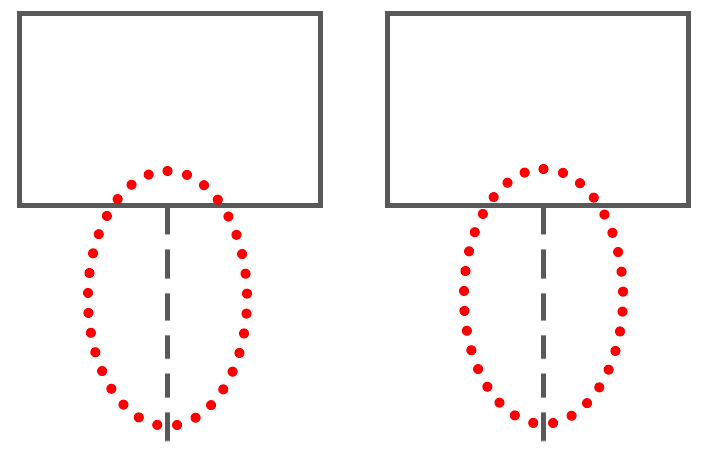
\includegraphics[width=2.3in]{uml-lifeline}} & lifeline &  Vertical dashed line representing the lifespan of the participant. Top is beginning of life, bottom is end. Life ends when the participant is deleted.\\
\raisebox{-\totalheight}{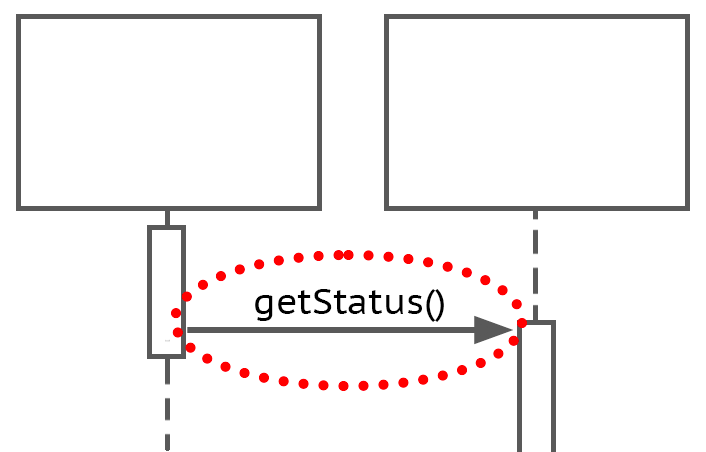
\includegraphics[width=2.3in]{uml-message}} & message & Interaction from one participant to another. Solid line with arrow. Often a method call.\\
\raisebox{-\totalheight}{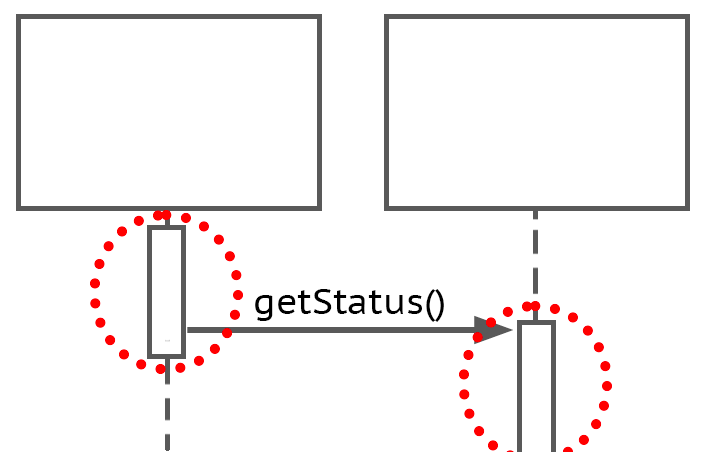
\includegraphics[width=2.3in]{uml-activation}} & activation & Box on lifeline indicating when the participant is active. Indicates method is on call stack.\\
\raisebox{-\totalheight}{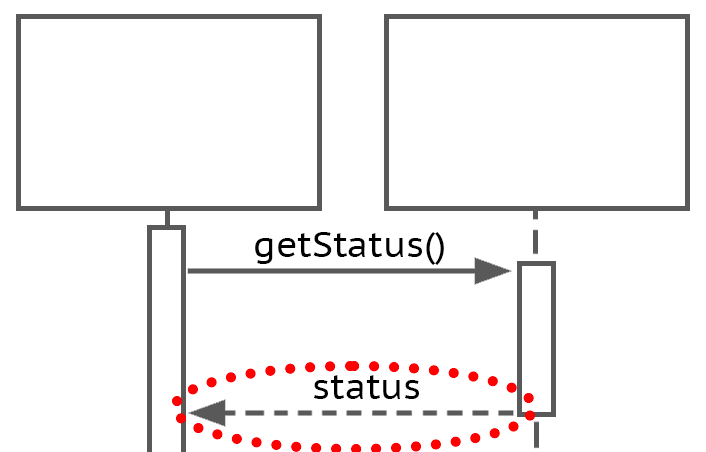
\includegraphics[width=2.3in]{uml-return}} & return & Dashed line with arrow indicating method return. Use only when it helps communicate something important about the interaction.\\
\end{tabular}

\rowcolors{2}{gray!25}{white}
\noindent\begin{tabular}{p{2.5in} p{1in} p{2.5in}}
\rowcolor{gray!25}
\raisebox{-\totalheight}{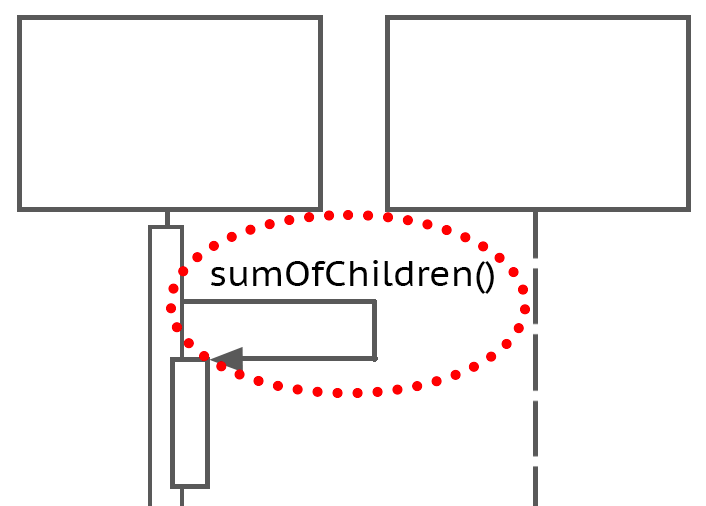
\includegraphics[width=2.3in]{uml-selfcall}} & self-call & Method calling self. Solid line with arrow pointing back to participant's own lifeline.\\
\raisebox{-\totalheight}{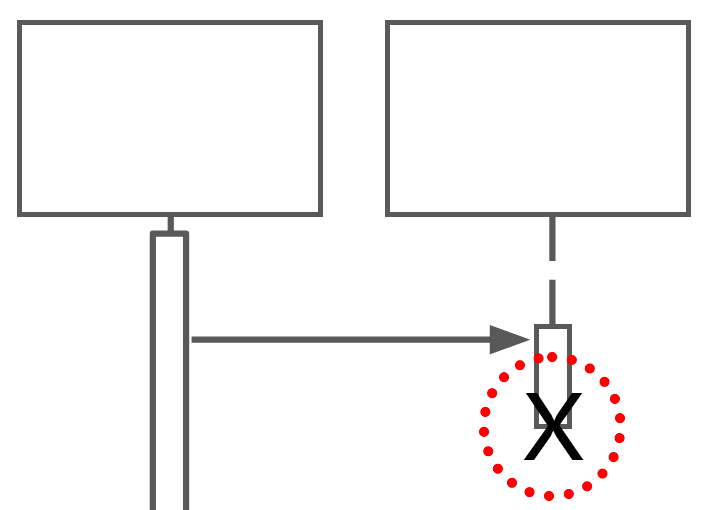
\includegraphics[width=2.3in]{uml-deletion}} & deletion & End of participant's life. Indicated by ``X'' on lifeline. \\
\end{tabular}

\section{Conclusion}
UML diagrams can be helpful for communicating how your code works. Class diagrams and sequence diagrams are two common-used types of UML diagrams. Each type of diagram emphasizes some part of the code design while leaving out other parts. This is because UML diagrams are for communicating with humans---not computers.

\section{Additional Resources}

\begin{description}
\item \fullcite{miles2006learning}
\item \fullcite{fowler2003uml}
\end{description}